%\large\zihao{-4}
%-----------------------------------------
\begin{center}
	{\heiti\bf\LARGE\zihao{3}{\biaoti\\}}
%	{\bf\LARGE\zihao{3}{\enbiaoti\\}}
%	{\enbiaoti}
	
	\vspace{0.3cm}
	{\heiti\bf\LARGE\zihao{-4}\minzi}
	
	{\zihao{5}\university\school,\city}
	
	{\zihao{5}zhongshengyanzy@foxmail.com}
\end{center}

%------------------------------------

%\begin{center}
%\begin{minipage}[t]{7cm}
\noindent{\zihao{5}{\bf 摘要:}
	\fangsong
	% 请填入中文摘要:
	本文介绍了信源编码在信息论中的重要性和应用。我们探讨了编码的基本概念和目的,并详细讨论了三种常用的信源编码方法:哈夫曼编码、香农编码和费诺编码。哈夫曼编码通过变长编码实现高效的数据压缩,香农编码是一种最优编码方法,费诺编码则是一种简单而有效的编码方法。
	我们比较了这些编码方法的特点和适用场景,并展望了未来的发展方向,包括非均匀信源编码、多媒体数据编码、自适应编码和结合信道编码等方面的研究挑战和前景。通过本文的研究,读者可以更好地理解信源编码的原理和方法,以及在实际应用中选择合适的编码方案来实现高效的数据压缩和传输。
}\vspace{0.1cm}
%\end{minipage}
%\end{center}
%\end{multicols}
%\begin{multicols}{2} 
\begin{multicols}{2} 
\section{引言}\label{chpt:1}%===============================================
在当今信息时代,数据的传输和存储成为了人们生活和工作中不可或缺的一部分。随着数据量的不断增长,有效地表示、压缩和传输数据变得至关重要。信息论是研究信息的表示、传输和处理的重要领域,广泛应用于通信、数据压缩和数据存储等领域。信源编码作为信息论的核心技术之一,通过有效地压缩和编码数据,可以显著提高数据传输的效率和可靠性。不同的信源编码方法具有各自的优点和局限性,因此对这些方法进行深入研究和比较分析,对于选择适当的编码方法和优化系统性能具有重要意义。

信源编码旨在通过对源数据进行压缩和编码,以减少数据的表示和传输所需的比特数。其目的是在保持数据内容准确的同时,实现数据的高效传输和存储。信源编码的应用涵盖了多个领域,如无线通信、图像和视频压缩、存储系统和互联网传输等。

本论文将着重介绍信源编码的概念、目的和基础,以及常用的信源编码方法,包括哈夫曼编码、算术编码和LZ编码。通过深入探讨这些编码方法的原理、特点和应用场景,我们旨在帮助读者更好地理解信源编码的核心概念和工作原理,并为实际应用提供指导。

在本文的第一部分,我们将简要介绍信息论和编码的基本概念,探讨信息论在数据传输和压缩中的重要性。然后,我们将深入探讨信源编码的目的和基础,包括无失真信源编码定理和限失真信源编码定理,这些理论为我们理解信源编码的原理和应用提供了基础。

接下来,我们将重点关注三种经典的信源编码方法:霍夫曼编码、算术编码和字典编码。霍夫曼编码以出现频率较高的符号使用较短的编码,而低频率的符号使用较长的编码,从而实现了高效的数据压缩。算术编码则基于符号的概率分布来动态地调整编码的长度,从而实现更高的压缩率。字典编码则通过构建和使用字典来实现对数据的编码和解码。我们将详细介绍每种编码方法的原理、编码过程和解码过程,并分析它们在不同场景下的优点和限制。通过比较这些编码方法的优缺点,我们将为研究者和工程师提供更好的理解和指导,以便在实际应用中做出明智的选择。

其次,在研究和比较各种信源编码方法后,我们将进行性能比较和分析,以客观评估不同编码方法的优劣。我们将客观评价不同编码方法的性能。此外,我们还将探讨这些编码方法在不同数据类型和传输环境下的适用性和实际应用效果。这将为研究者和工程师提供有价值的见解,以在实际应用中权衡利弊并做出明智的决策。

最后,我们将总结各种信源编码方法的特点和适用场景,并提出未来的研究方向和改进的建议。通过本论文的研究和分析,我们希望能够为信源编码领域的进一步发展提供新的思路和启示,以满足日益增长的信息传输需求,并提高通信系统的效率和可靠性。让我们开始探索信源编码的奥秘,揭示其中的原理和方法,为信息的传输和处理打开新的大门。

%\end{multicols}
%
%\begin{figure}[H]
%	\centering
%	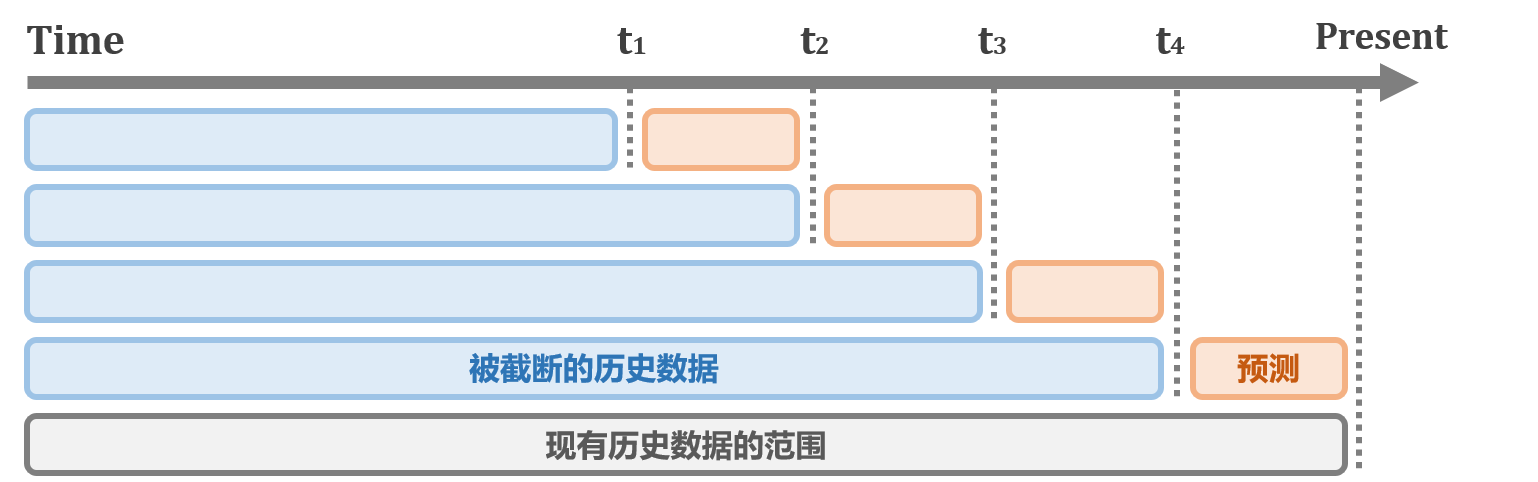
\includegraphics[width=14cm]{pics/bt1.png}\\
%	\caption{时间序列扩展窗口回测的概念示意图}\label{fig:backtest1}
%\end{figure}
%
%\begin{multicols}{2} 

%
%\begin{table}[H]
%	%\scriptsize
%	\footnotesize
%	\renewcommand{\arraystretch}{1.0}
%	\centering
%	\caption{\centering 模型的前移验证的预测评价指标统计对比}\label{tb:8}
%	\begin{tabular}{cccc}
%		\toprule[1.5pt]
%		&ARIMA&指数平滑&Prophet\\
%		\midrule[1pt]
%		 RMSE的中位数& 0.5440 &0.4785&\textbf{0.4055}\\
%		 RMSE的平均数& 0.5169&0.4529& \textbf{0.4126} \\
%		 MAE的中位数&0.4530 & 0.3435&\textbf{0.3045}\\
%		 MAE的平均值&0.4411 &\textbf{0.4115}&0.4116\\
%		 MAPE的中位数&108.84&92.38&\textbf{73.21}\\
%		 MAPE的平均值&134.32&119.56&\textbf{85.55}\\
%		\bottomrule[1.5pt]
%	\end{tabular}
%\end{table}
\section{信源编码基础}
在本部分中,我们将深入研究信源编码的基础知识,包括信源编码的概念、无失真信源编码定理和限失真信源编码定理。通过理解这些基础概念,我们可以更好地理解信源编码的目的和原理。
\subsection{信源编码的概念}
信源编码是信息论中的重要概念,它涉及将源数据进行编码转换的过程,以减少所需传输或存储的比特数。信源编码的主要目的是实现高效的数据压缩,以便在传输或存储过程中节省带宽或存储空间。通过信源编码,我们可以将原始数据表示为更紧凑、更优化的编码形式,从而实现数据的高效传输和存储。

\begin{figure}[H]
	\centering
	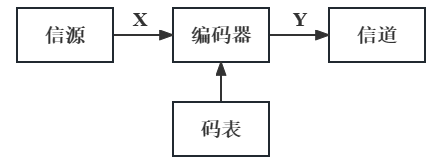
\includegraphics[width=0.85\linewidth]{pics/fig1}
	\caption{信源编码器示意图}
	\label{fig:fig1}
\end{figure}

信源编码的基本途径有两个,一是使序列中的各个符号尽可能地互相独立,即解除相关性;二是使编码中各个符号出现的概率尽可能地相等,即概率均匀化。主要是利用数据中的统计特性和冗余性来实现压缩。数据通常具有一定的统计规律,例如在文本数据中,某些字母或词汇出现的频率较高,而其他的则相对较少出现。信源编码的任务就是利用这些统计规律,对出现频率高的数据进行更短的编码,而对出现频率低的数据进行更长的编码,从而达到整体数据压缩的效果。

与信道编码不同,信源编码主要关注数据的压缩和表示,而不考虑传输过程中的误差纠正。信道编码主要应用于受到信道干扰和噪声的传输环境中,其目的是通过在发送端引入冗余信息,以提高数据的可靠性和抗干扰能力。相比之下,信源编码更加注重数据的压缩和优化,以减少所需的传输或存储资源。
\subsection{无失真信源编码定理}
\subsubsection{定长信源编码定理}
一个熵为$H(S)$的离散无记忆信源,若对其$N$次扩展信源进行等长$r$元编码,码长为$l$,对于任意$\varepsilon$大于0,只要满足
\begin{equation}
	\frac{l}{N} \geq \frac{H(S)+\varepsilon}{\log r}
\end{equation}
当$N\rightarrow \infty$时,则可以实现几乎无失真编码,反之,若:
\begin{equation}
	\frac{l}{N} \leq \frac{H(S)-2 \varepsilon}{\log r}
\end{equation}
则不可能实现无失真编码,当$N\rightarrow \infty$时,译码错误率接
近于1。为了衡量编码效果,引进
\begin{equation}
	\eta=\frac{H(S)}{R^{\prime}}=\frac{H(S)}{\frac{l}{N} \log r}
\end{equation}
称为编码效率。最佳编码效率为:
\begin{equation}
	\eta=\frac{H(S)}{R^{\prime}}=\frac{H(S)}{H(S)+\varepsilon} \quad \varepsilon=\frac{1-\eta}{\eta} H(S)
\end{equation}

\subsubsection{变长信源编码定理}
离散无记忆信源$S$的$N$次扩展信源$S^N$,其熵为$H(S^N)$,并且编码器的码元符号集为 $A:{\alpha_1,\alpha_2,...,\alpha_q}$ 对信源$S^N$进行编码,总可以找到一种编码方法,构成单义可译码,使信源$S$中每个符号$s_i$所需要的平均码长满足
\begin{equation}
	\frac{H(S)}{\log r} \leq \frac{L_{N}}{N}<\frac{H(S)}{\log r}+\frac{1}{N}
\end{equation}
当$N\rightarrow \infty$时,则得到
\begin{equation}
	\lim_{N\rightarrow \infty} \overline{L} = H_r(S)
\end{equation}
这个定理是香农信息论中非常重要的一个定理,它指出,要做到无失真的信源编码,信源每个符号所需要的平均码元数就是信源的熵值,如果小于这个值,则唯一可译码不存在,可见,熵是无失真信源编码的极限值。定理还指出,通过对扩展信源进行编码,当$N\rightarrow \infty$时,平均码长可趋近该极限值。

总结起来,无失真信源编码定理提供了在定长编码和变长编码情况下实现无失真信源压缩的理论保证。在实际应用中,我们可以根据源符号的统计特性和信息熵来选择合适的编码方案,以实现高效的数据压缩和无损数据的还原。
\subsection{限失真信源编码定理}
除了无失真信源编码定理之外,信息论中还存在一个重要的定理,即限失真信源编码定理。该定理考虑了在信源编码过程中引入一定程度的失真,并给出了在给定失真约束下实现最优信源编码的方法。
\begin{figure}[H]
	\centering
	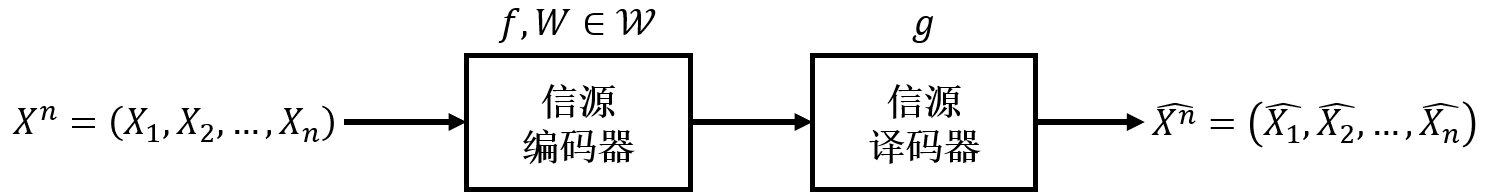
\includegraphics[width=0.95\linewidth]{pics/xinyuan}
	\caption{限失真信源编码模型}
	\label{fig:xinyuan}
\end{figure}
\subsubsection{失真函数的定义}
在限失真信源编码定理中,我们首先需要定义失真函数,它用来衡量信源编码的失真程度。失真函数通常定义为原始数据与解码数据之间的平均差异或距离。一种常见的失真函数是均方误差,用来衡量信源编码后的数据与原始数据之间的均方差。

设源符号集合$S$中的每个符号$s$对应的编码为$C(s)$,解码器将编码$C(s)$映射回原始符号$s'$。失真函数$D(s, s')$衡量了原始符号$s$与解码符号$s'$之间的差异。

\subsubsection{限失真信源编码定理}
限失真信源编码定理的核心思想是在给定的失真约束条件下,寻找一种编码方案,使得失真函数达到最小。定理的表述如下:

对于给定的失真约束$D_{max}$,对于具有$n$个符号的源符号集合$S$,如果存在一个编码方案,使得平均失真$D(S)$满足$D(S)\leq D_{max}$,同时满足数据传输速率$R\leq C(D_{max})$,其中$C(D_{max})$为失真约束下的信道容量,则该编码方案可以实现限失真信源编码。换句话说,在给定的失真约束下,限失真信源编码定理保证了可以找到一种编码方案,使得平均失真不超过预设的失真约束,并且数据传输速率不超过失真约束下的信道容量。

限失真信源编码定理在实际应用中具有广泛的意义。在许多情况下,我们不能要求完全无失真的信源编码,因为这通常会导致较低的数据压缩率。相反,我们需要在允许一定失真的前提下,选择合适的编码方案以平衡压缩效率和数据质量。限失真信源编码定理提供了一种理论基础,通过优化失真函数和数据传输速率之间的关系,我们可以设计出适合不同失真约束的信源编码方案。例如,在音频和图像压缩中,我们通常允许一定的失真,以换取更高的压缩率。通过限失真信源编码定理,我们可以根据特定应用场景的失真需求,选择合适的失真函数和失真约束,并设计出相应的信源编码方案。

在实际应用中,常见的限失真信源编码方法包括基于率失真优化(Rate-Distortion Optimization)的编码算法。这类算法通过在失真函数和数据传输速率之间进行权衡,寻找最优的编码方案。通过限失真信源编码定理的研究和应用,我们能够实现在失真约束下的最优信源编码,有效平衡数据压缩和数据质量的需求。这在多媒体数据压缩、图像处理、音频传输等领域具有重要的实际意义。

\section{常用的信源编码方法}
\subsection{哈夫曼编码}
哈夫曼编码是一种常用的无失真信源编码方法,它通过根据源符号出现的概率来构建最优的变长编码方案。哈夫曼编码具有简单高效的特点,广泛应用于数据压缩和信息传输领域。

\subsubsection{编码过程}

哈夫曼编码的编码过程包括以下几个步骤:
\begin{enumerate}
	\item[(1)] 统计源符号的概率:对给定的源符号集合进行统计,计算每个符号出现的概率。概率可以根据符号在数据中出现的频率进行估计。
	
	\item[(2)] 构建哈夫曼树:根据源符号的概率构建哈夫曼树。哈夫曼树是一种特殊的二叉树,其中每个叶节点表示一个源符号,而每个非叶节点表示两个子节点的概率之和。构建哈夫曼树的方法通常是通过贪心算法,从概率最小的两个节点开始逐步构建。
	
	\item[(3)] 分配编码:从哈夫曼树的根节点开始,沿着树的路径向下,为每个叶节点分配编码。左子树路径上的编码为0,右子树路径上的编码为1。最终,每个源符号都有一个唯一的变长编码。
	
	\item[(4)] 生成编码表:将每个源符号和其对应的编码记录在编码表中。编码表可以用于编码和解码过程。
	
	\item [(5)] 编码数据:根据生成的编码表,将原始数据中的每个符号替换为其对应的编码。编码后的数据将具有较短的平均编码长度。
\end{enumerate}
\begin{figure}[H]
	\centering
	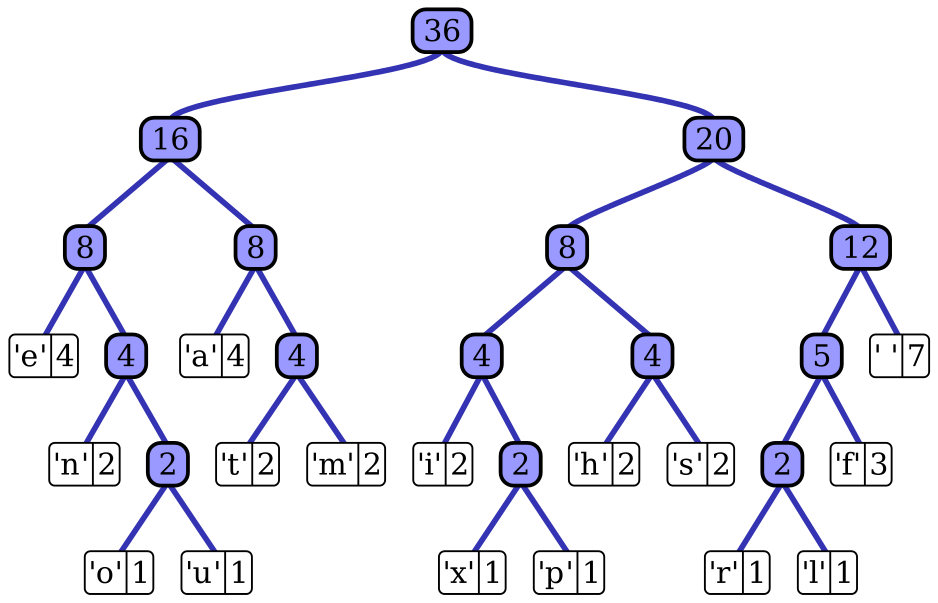
\includegraphics[width=0.7\linewidth]{pics/Huffman_tree_2.svg}
	\caption{哈夫曼编码示意图}
	\label{fig:huffmantree2}
\end{figure}

哈夫曼编码的效果取决于源符号的概率分布。当源符号的概率分布接近均匀分布时,哈夫曼编码可以达到最佳效果,即平均编码长度接近信息熵。哈夫曼编码的优势在于能够根据不同源符号的出现概率分配不同长度的编码,使得频率较高的符号具有较短的编码长度,而频率较低的符号具有较长的编码长度。这样可以最大程度地减小编码的平均长度,提高数据的压缩效率。

\subsubsection{哈夫曼编码示例}
\noindent 例:有一单符号离散无记忆信源,对该信源进行二进制哈夫曼编码。
\begin{figure}[H]
	\centering
	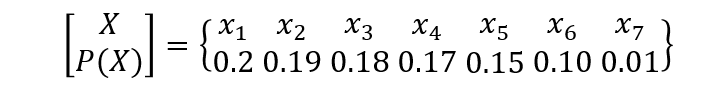
\includegraphics[width=0.95\linewidth]{px}
	\label{fig:px}
\end{figure}
哈夫曼编码结果如下图所示:
\begin{figure}[H]
	\centering
	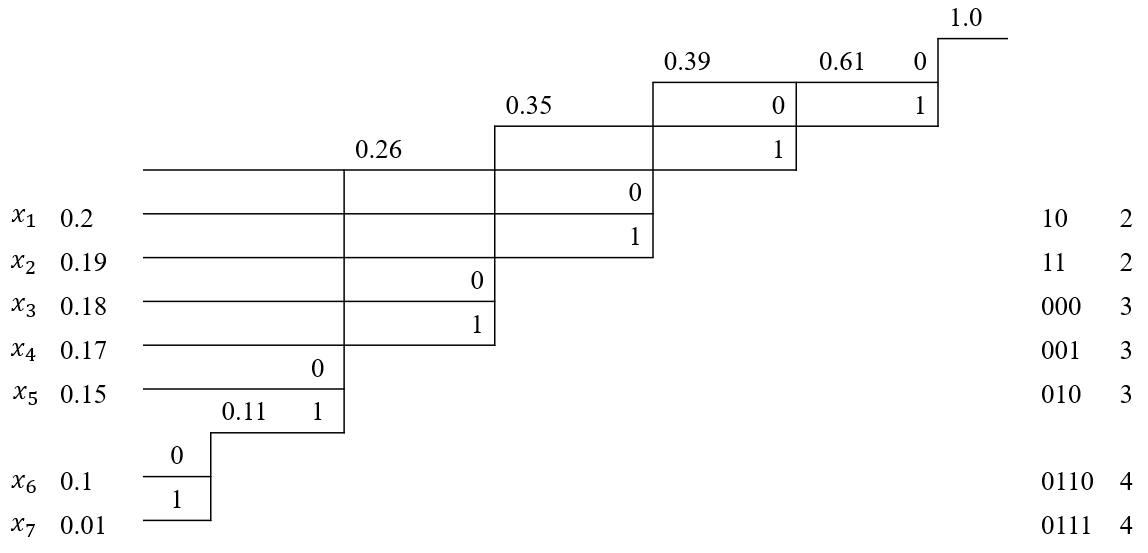
\includegraphics[width=0.95\linewidth]{pics/xian1}
	\caption{哈夫曼编码结果}
	\label{fig:xian1}
\end{figure}
\begin{itemize}
	\item 计算出给定信源香农码的平均码长:
	
	$\bar{L}=\sum_{i=1}^{7} p\left(x_{i}\right) k_{i}=2.72$比特/信源符
	
	\item 由离散无记忆信源熵定义,可计算出:
	
	$H(X)=-\sum_{i=1}^{7} p\left(x_{i}\right) \log p\left(x_{i}\right)=2.61$
	
	\item 由离散无记忆信源熵定义,可计算出:
	
	$H(X)=-\sum_{i=1}^{7} p\left(x_{i}\right) \log p\left(x_{i}\right)=2.72$
	\item 编码效率为信源熵和信息率之比,则
	
	$\eta=\frac{2.61}{2.72}=95.9\%$
\end{itemize}
\subsubsection{特点和应用}
哈夫曼编码具有以下特点和应用:
\begin{itemize}
	\item 变长编码:哈夫曼编码生成的编码是变长的,不同符号的编码长度不同,可以根据
	
	\item 无前缀码:哈夫曼编码是一种无前缀码,即任何一个编码不是其他编码的前缀。这样可以确保在解码时不会出现歧义,每个编码都能被唯一解码。
	
	\item 数据压缩:哈夫曼编码在数据压缩领域得到广泛应用。通过根据源符号的概率分布生成最优的编码方案,可以实现较高的数据压缩比。哈夫曼编码被用于无损压缩算法中,如ZIP文件压缩。
	
	\item 图像和音频压缩:由于图像和音频数据通常具有一定的冗余性,哈夫曼编码被广泛应用于图像和音频压缩中。通过将频率较高的图像或音频符号用较短的编码表示,可以有效减小数据的存储空间和传输带宽。
\end{itemize}
总而言之,哈夫曼编码是一种常用的无失真信源编码方法,通过根据源符号的概率分布生成最优的变长编码方案,实现高效的数据压缩和传输。它在数据压缩、图像处理、音频传输和通信系统等领域都具有重要的应用价值。

\subsection{香农编码}
香农编码,也称为最佳编码或熵编码,是一种常用的无失真信源编码方法,由克劳德·香农于1948年提出。它通过基于源符号的概率分布来生成最优的编码方案,以达到最小的平均编码长度。
\subsubsection{编码过程}
\begin{enumerate}
	\item[(1)] 将信源符号按概率从大到小的顺序排列, 为方便起见, 令  $p\left(x_{1}\right) \geq p\left(x_{2}\right) \geq \cdots \geq p\left(x_{n}\right)$ 
	
	\item[(2)] 令  $p\left(x_{0}\right)=0$ , 用 $ p a\left(x_{j}\right), j=i+1 $ 表示第 $i$ 个码字的累加概率, 则:
	$p_{a}\left(x_{j}\right)=\sum_{i=0}^{j-1} p\left(x_{i}\right), j=1,2, \cdots, n$
	\item[(3)] 确定满足下列不等式的整数  $k_{i}$ , 并令$k_{i}$为第$i$个码字的长度
	
	$-\log _{2} p\left(x_{n}\right) \leq k_{i}<-\log _{2} p\left(x_{n}\right)+1 $
	
	\item[(4)] 将  $p_{a}\left(x_{i}\right)$ 用二进制表示, 并取小数点后 $k_{i}$ 位作为符号 $x_{i}$ 的编码。
\end{enumerate}
\subsubsection{香农编码示例}
仍以3.1.2的例子为例,进行香农编码。结果见下表:
\begin{table}[H]
	%\scriptsize
	\footnotesize
	\renewcommand{\arraystretch}{1.0}
	\centering
	\begin{tabular}{cccccc}
			\toprule[1.5pt]
			信源符号 & 符号概率 & 累加概率 & log2 & 码长 & 码字     \\
			\midrule[1pt]
			x1   & 0.2  & 0    & 2.32 & 3  & 0      \\
			x2   & 0.19 & 0.2  & 2.4  & 3  & 1      \\
			x3   & 0.18 & 0.39 & 2.47 & 3  & 11     \\
			x4   & 0.17 & 0.57 & 2.56 & 3  & 100    \\
			x5   & 0.15 & 0.74 & 2.74 & 3  & 101    \\
			x6   & 0.1  & 0.89 & 3.32 & 4  & 1110   \\
			x7   & 0.01 & 0.99 & 6.44 & 7  & 111110 \\
			\bottomrule[1.5pt]
	\end{tabular}
	\caption{\centering 香农编码结果}\label{tb:8}
\end{table}
\begin{itemize}
	\item 计算出给定信源香农码的平均码长:
	
	$\bar{L}=\sum_{i=1}^{7} p\left(x_{i}\right) k_{i}=3.14$比特/信源符
	
	\item 由离散无记忆信源熵定义,可计算出:
	
	$H(X)=-\sum_{i=1}^{7} p\left(x_{i}\right) \log p\left(x_{i}\right)=2.61$
	
	\item 
	采用香农编码的信息率为
	
	$R^{\prime}=\frac{\bar{L}_1}{N} \log _2 r=\frac{3.14}{1} \log _2 2=3.14$
	\item 编码效率为信源熵和信息率之比,则
	
	$\eta=\frac{2.61}{3.14}=83.1\%$
\end{itemize}
显而易见,香农编码的效率并不是很高。

\subsection{费诺编码}
\subsubsection{编码过程}
\begin{enumerate}
	\item[(1)] 将信源符号按概率从大到小的顺序排列, 为方便起见, 令 $p\left(x_1\right) \geqslant p\left(x_2\right) \geqslant \cdots \geqslant p\left(x_n\right)$。
	
	\item[(2)] 按编码进制数将概率分组, 使每组概率尽可能接近或相等。如编二进制码就分成两组, 编 $m$ 进制码就分成 $m$ 组。
	
	\item[(3)] 给每一组分配一位码元。
	
	\item[(4)] 将每一分组再按同样原则划分, 重复步骤2和3, 直至概率不再可分为止。
\end{enumerate}

\subsubsection{费诺编码举例}
同样对前文的例子进行费诺编码:
\begin{figure}[H]
	\centering
	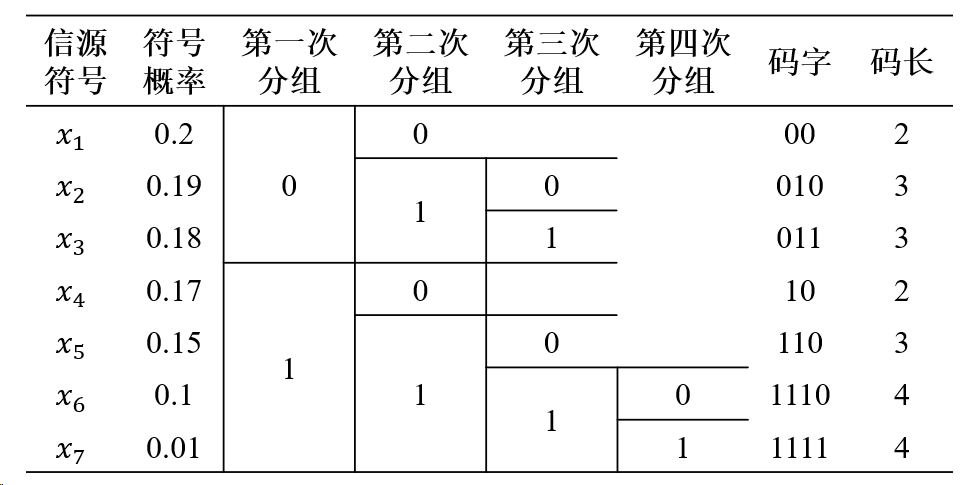
\includegraphics[width=0.95\linewidth]{screenshot001}
	\caption{费诺编码结果}
	\label{fig:screenshot001}
\end{figure}
\begin{itemize}
	\item 计算出给定信源香农码的平均码长
	
	$\bar{L}=\sum_{i=1}^7 p\left(x_i\right) k_i=2.74 \quad \text{bit/信源符号}$
	
	\item 由离散无记忆信源樀定义, 可计算出:
	$H(X)=-\sum_{i=1}^7 p\left(x_i\right) \log p\left(x_i\right)=2.61$ bit/信源符号
	
	\item 采用香农编码的信息率为
	$$R^{\prime}=\frac{\overline{L_1}}{N} \log _2 r=\frac{2.74}{1} \log _2 2=2.74, \quad N=1, r=2 $$
	
	\item 编码效率为信源嫡和信息率之比。则 
	
	$\eta=\frac{2.61}{2.74}=95.3 \%$。
\end{itemize}
可看出,本例中费诺编码有较高的编码效率。费诺码比较适合于每次分组概率都很接近的信源。特别是对每次分组概率都相等的信源进行编码时,可达到理想的编码效率。
\section{总结与展望}
\subsection{结论}

信源编码是信息论中的重要领域,旨在通过优化编码方案实现对数据的高效压缩和传输。在本文中,我们首先介绍了编码的基本概念和作用,包括无失真信源编码和限失真信源编码的定理基础。无失真信源编码定理强调了通过变长编码可以实现平均编码长度的最小化,而限失真信源编码定理考虑了在限定失真度的情况下进行编码的问题。

我们详细介绍了三种常用的信源编码方法:哈夫曼编码、香农编码和费诺编码。哈夫曼编码是一种变长编码方法,通过根据符号出现的概率分配不同长度的编码,实现了较高的数据压缩比。香农编码是一种最优编码方法,通过根据源符号的概率分布生成最小平均编码长度的方案。费诺编码是一种无失真编码方法,通过二分法逐步分组编码,实现了有效的数据压缩。

每种编码方法都有其特点和适用场景。哈夫曼编码适用于频率不均衡的信源数据,能够实现较高的压缩效率。香农编码是一种最优编码方法,适用于源符号概率已知的情况,能够接近信息熵并实现较高的压缩比。费诺编码是一种简单而有效的编码方法,适用于相对均衡的信源数据,可以实现较好的数据压缩效果。

\subsection{展望未来的发展方向和研究挑战}

信源编码作为信息论中的重要领域,在数据压缩和通信领域发挥着关键作用。然而,随着数据量的不断增大和多样化的应用需求,仍然存在一些挑战和研究方向值得探索。

未来的研究可以集中在以下方面:
\begin{itemize}
	\item 非均匀信源编码:针对非均匀信源数据的编码方法研究可以进一步研究非均匀信源编码方法,以解决频率不均衡的信源数据问题。这包括对于具有长尾分布的信源数据的编码方案的研究和优化,以提高对于低频符号的编码效率。
	
	\item 多媒体数据编码:随着多媒体数据的广泛应用,对于音频、图像和视频等多媒体数据的高效编码成为一个重要的研究方向。研究人员可以探索针对不同类型多媒体数据的特点和压缩需求,开发更加高效的编码算法和技术。
	
	\item 自适应编码:传统的信源编码方法在编码过程中需要准确的概率分布信息,然而实际应用中概率分布可能随时间变化或未知。因此,自适应编码成为一个重要的研究方向,旨在根据实时数据的统计信息和特征来动态调整编码方案,以提高编码效率和适应性。
	
	\item 结合信道编码:信道编码和信源编码是信息传输中不可或缺的两个环节。未来的研究可以探索如何将信道编码和信源编码相结合,实现编码的联合优化,从而在数据传输中获得更好的性能和可靠性。
\end{itemize}

综上所述,信源编码是信息论中重要的技术之一,具有广泛的应用。未来的研究将聚焦于非均匀信源编码、多媒体数据编码、自适应编码和结合信道编码等方面,以推动信源编码在数据压缩和通信领域的进一步发展和应用。
\end{multicols}




















